
\documentclass{bredelebeamer}




%%%%%%%%%%%%%%%%%%%%%%%%%%%%%%%%%%%%%%%%%%%%%%%%



\title[SVM avec Python]{Séparateurs à Vaste Marge }
% Titre du diaporama

\subtitle{SVM avec Python}
% Sous-titre optionnel

\author{\\
MARHOUN  Marouane\\ 
$\hspace*{0.3 cm}$ ECH-CHOUYYEKH  Monir \vspace{2\baselineskip}\\
Encadrer par :\\
 Mr. CHRAYEH Mohamed }
% La commande \inst{...} Permet d'afficher l' affiliation de l'intervenant.
% Si il y a plusieurs intervenants: Marcel Dupont\inst{1}, Roger Durand\inst{2}
% Il suffit alors d'ajouter un autre institut sur le modèle ci-dessous.

\institute[ENSA]
{Université Abdelmalek Essaadi \\
École Nationale des Sciences Appliquées
  }


\date{26 novembre 2018}
% Optionnel. La date, généralement celle du jour de la conférence

\subject{}
% C'est utilisé dans les métadonnes du PDF



\logo{

\includegraphics[scale=0.15]{22.png} % logo
}



%%%%%%%%%%%%%%%%%%%%%%%%%%%%%%%%%%%%%%%%%%%%%%%%%%%%%%%%%%%%%%%%%%%%%


%%%%%%%%%%%%%%%%%%%%%%%%%%%%%%%%%%%%%%%%%%%%%%%%%%%%%%%%%%%%%%%%%%%%%
\begin{document}

\begin{frame}
  \titlepage
\end{frame}





\begin{frame}{Plan}
  \tableofcontents
  % possibilité d'ajouter l'option [pausesections]
\end{frame}




\section{Introduction}

\begin{frame}{Introduction}

 L’apprentissage automatique (Machine Learning ML) apprend un modèle à partir des données passées afin de prédire les données futures. Le processus clé est l’apprentissage, qui est l’une des intelligences artificielles. De nombreuses techniques statistiques, probabilistes et d’optimisation différentes peuvent être mises en œuvre comme méthodes d’apprentissage telles que la régression logistique, les réseaux de neurones artificiels (RNA), K-voisin le plus proche (KNN), arbre de décision (DT), Naïve Bayes et Séparateurs à Vaste Marge (SVM).\\

\begin{center}  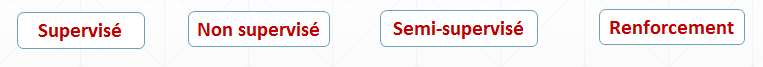
\includegraphics[scale=0.45]{27.png} \end{center}
\vfill
 \end{frame}
   

 
\subsection{Domaine d'application}
\begin{frame}{Introduction}
La technologie de reconnaissance faciale « par exemple » permet aux plateformes de médias sociaux d'aider les utilisateurs à marquer et partager des photos d'amis.\vspace{2\baselineskip}
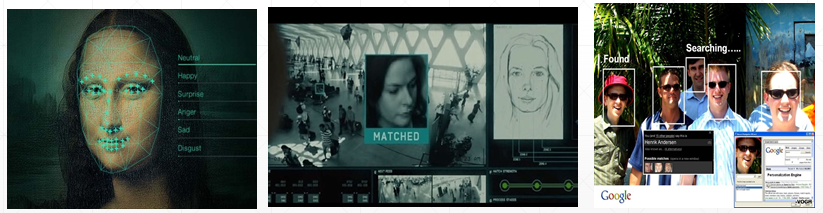
\includegraphics[scale=0.5]{1.png}	
\end{frame}

\begin{frame}{Introduction}
La technologie de reconnaissance optique des caractères (OCR) convertit les images du texte en caractères mobiles.
\vfill
\begin{center} 
\includegraphics[scale=0.6]{2.png} \end{center}
\vfill
 \end{frame}  
 
\section{ SVM}
\begin{frame}{SVM}	
\begin{itemize}
		\item Support Vector Machines est considéré comme une approche de classification, mais peut être utilisé dans les deux types de problèmes de classification et de régression.
		\item Méthode relativement récente qui découle de premiers travaux théoriques de Vapnik et Chervonenkis en 1995, démocratisés à partir de 2000.
		\item L’idée est de rechercher une règle de décision basée sur \textcolor{red}{une séparation par hyperplan de marge optimale.}
		\item Le principe de l’algorithme est d’intégrer lors de la phase d’apprentissage une estimation de sa complexité pour limiter le phénomène d’over-fitting.
	\end{itemize}
   \end{frame}
   
\subsection{Classification}
\begin{frame}{SVM}
Une machine à vecteurs de support (SVM) effectue la classification en recherchant l'hyperplan qui optimise la marge entre les deux classes. Les vecteurs (cas, points) qui définissent l'hyperplan sont les vecteurs de support.on définit Algorithme par les étapes:\vspace{1\baselineskip}\\
  \frametitle{Séparateurs à Vaste Marge SVM }
\begin{minipage}{0.4\textwidth}
     \begin{itemize}
        \item Définir un hyperplan optimal: maximiser la marge
        \item Pour les problèmes séparables de manière non linéaire: prévoir un terme de pénalité pour les erreurs de classification.
        \item Mappez les données vers un espace de grande dimension où il est plus facile de classer avec des surfaces de décision linéaires: reformulez le problème afin que les données soient mappées implicitement dans cet espace.
\end{itemize}
    \end{minipage}
    \begin{minipage}{0.4\textwidth}
    $ \hspace*{10 cm}$     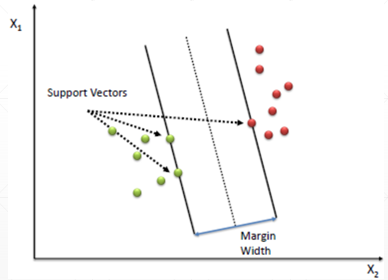
\includegraphics[scale=0.45]{3.png}
    \end{minipage}
\end{frame}

\subsection{Régression}
\begin{frame}{SVM}
    La régression vectorielle de support (SVR) utilise les mêmes principes que la SVM pour la classification, avec seulement quelques différences mineures.\\
\begin{itemize}
         \item En cas de régression, une marge de tolérance (epsilon) est définie comme une approximation du SVM qui l'aurait déjà demandé au problème.
         \item L'idée principale est toujours la même: minimiser les erreurs, individualiser l'hyperplan qui maximise la marge, en gardant à l'esprit qu'une partie de l'erreur est tolérée.
\end{itemize}
\vfill
\begin{center} 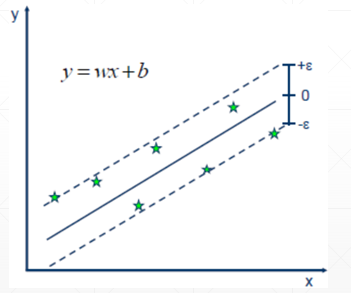
\includegraphics[scale=0.5]{4.png} \end{center}
\vfill
\end{frame}

\section{Séparation linéaire par SVM}
\subsection{Notion de base }
\begin{frame}{Séparation linéaire par SVM}
Les termes que nous allons utiliser fréquemment dans ce travail:
\begin{itemize} 
        \item \textcolor{red}{Noyau}: fonction utilisée pour mapper une donnée de dimension inférieure en une donnée de dimension supérieure.
        \item \textcolor{red}{Hyper plan}: en SVM, il s’agit essentiellement de la ligne de séparation entre les classes de données. Bien que dans SVR nous allons le définir comme la ligne qui nous aidera à prédire la valeur continue ou la valeur cible.
        \item \textcolor{red}{Ligne de limite}: Dans SVM, deux lignes autres que Hyper Plan créent une marge. Les vecteurs de support peuvent se trouver sur les lignes de délimitation ou à l’extérieur. Cette ligne de démarcation sépare les deux classes. En SVR, le concept est le même.
        \item \textcolor{red}{Vecteurs de support}: Ce sont les points de données les plus proches de la limite. La distance des points est minimale ou minimale.        
\end{itemize}
\end{frame}

\subsection{Cas linéairement séparable }
\begin{frame}{Séparation linéaire par SVM}
Nous avons besoin de présenté une technique permettant de construire un hyperplan de séparation optimal entre deux classe parfaitement séparer (linéairement séparable).\vspace{2\baselineskip}

Le problème abordé est celui de la discrimination binaire. Il s’agit de trouver un moyen permettant de construire une fonction de décision associant à chaque observation sa classe. Alors L’idée des SVMs est de rechercher un hyperplan (droite dans le cas de deux dimensions) qui sépare le mieux ces deux classes (1 et -1 ou + et  -), soit  $x_{i}$=($x_{1}$,$x_{2}$,…,$x_{n}$) est l’ensembles des données et $ y_{i}\in\{-1,1\} $  est la classe de chacune.\vspace{2\baselineskip}


L’objectif est de trouver une séparation linéaire permettant de distinguer les ‘+’ des ‘-’. Le classifieur (fonction de discrimination) se présente sous la forme d’une combinaison linéaire des variables.
\end{frame}

\begin{frame}{Séparation linéaire par SVM}
\textcolor{red}{Classificateurs Linéaires}
%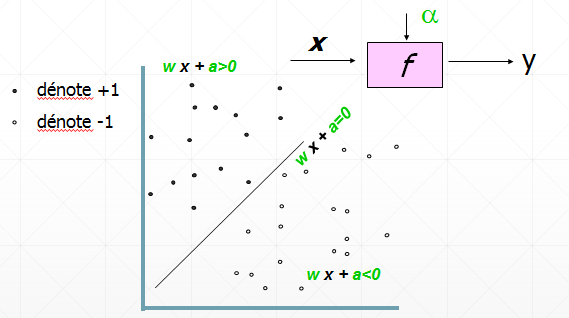
\includegraphics[scale=0.6]{5.png}
 
    \frametitle{Séparation linéaire par SVM }
    \begin{minipage}{0.3\textwidth}
        Comment classeriez-vous ces données?\vspace{2\baselineskip}
        
        
        f(x,w,a) = sign($w^{T}$ x + a)
    \end{minipage}
    \begin{minipage}{0.3\textwidth}
        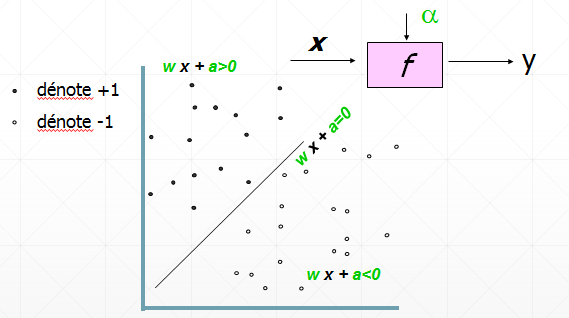
\includegraphics[scale=0.55]{5.png}
    \end{minipage}
\end{frame}

\begin{frame}{Séparation linéaire par SVM}
\textcolor{red}{Classificateurs Linéaires}
%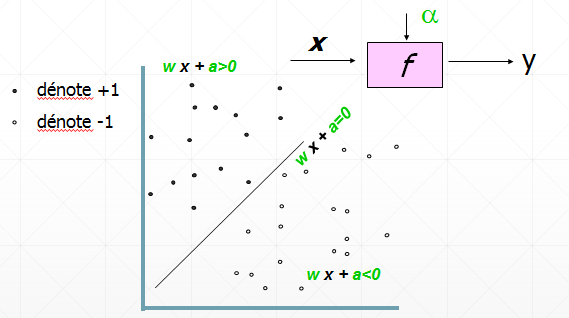
\includegraphics[scale=0.6]{5.png}
 
    \frametitle{Séparation linéaire par SVM }
    \begin{minipage}{0.3\textwidth}
        Comment classeriez-vous ces données?\vspace{2\baselineskip}
        
        
        f(x,w,a) = sign($w^{T}$ x + a)
    \end{minipage}
    \begin{minipage}{0.3\textwidth}
        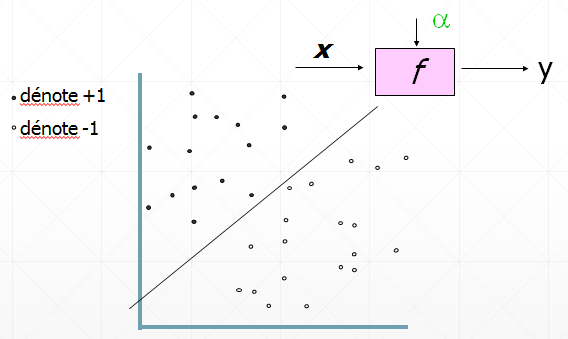
\includegraphics[scale=0.55]{6.png}
    \end{minipage}
\end{frame}


\begin{frame}{Séparation linéaire par SVM}
\textcolor{red}{Classificateurs Linéaires}
%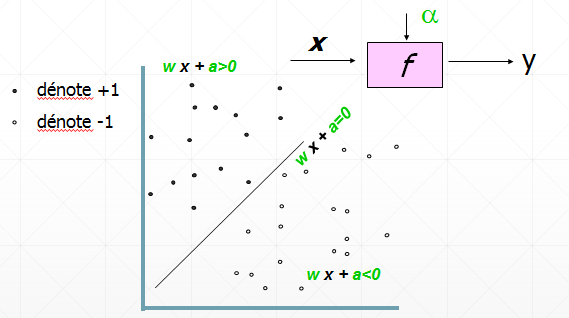
\includegraphics[scale=0.6]{5.png}
 
    \frametitle{Séparation linéaire par SVM }
    \begin{minipage}{0.3\textwidth}
        Comment classeriez-vous ces données?\vspace{2\baselineskip}
        
        
        f(x,w,a) = sign($w^{T}$ x + a)
    \end{minipage}
    \begin{minipage}{0.3\textwidth}
        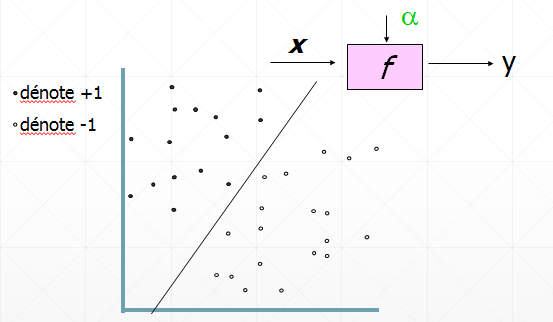
\includegraphics[scale=0.55]{7.png}
    \end{minipage}
\end{frame}

\begin{frame}{Séparation linéaire par SVM}
\textcolor{red}{Classificateurs Linéaires}
%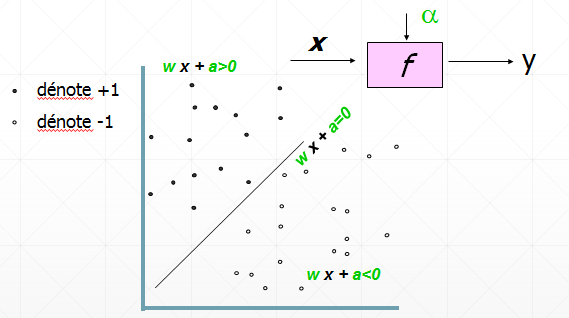
\includegraphics[scale=0.6]{5.png}
 
    \frametitle{Séparation linéaire par SVM}
    \begin{minipage}{0.3\textwidth}
     N'importe lequel de ces serait bien ..
..mais qui est le meilleur?
\vspace{2\baselineskip}
        
        
        f(x,w,a) = sign($w^{T}$ x + a)
    \end{minipage}
    \begin{minipage}{0.3\textwidth}
        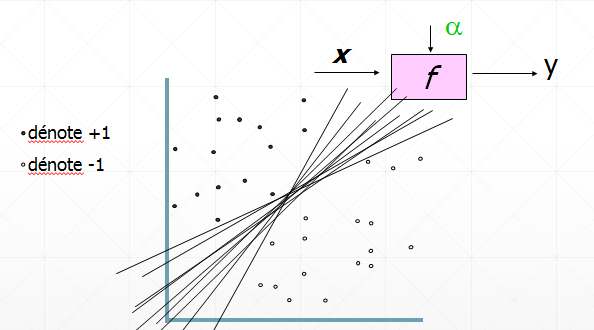
\includegraphics[scale=0.55]{8.png}
    \end{minipage}
\end{frame}


\begin{frame}{Séparation linéaire par SVM}
\textcolor{red}{Classificateurs Linéaires}
%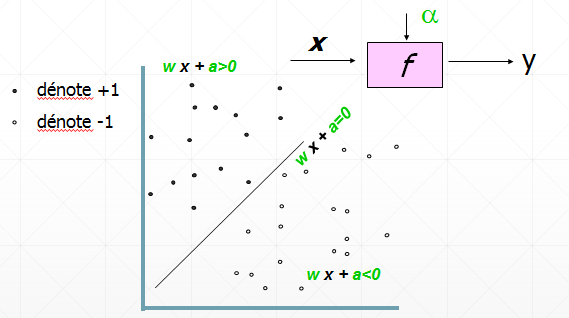
\includegraphics[scale=0.6]{5.png}
 
    \frametitle{Séparation linéaire par SVM }
    \begin{minipage}{0.3\textwidth}
        Comment classeriez-vous ces données?\vspace{2\baselineskip}
        
        
        f(x,w,a) = sign($w^{T}$ x + a)
    \end{minipage}
    \begin{minipage}{0.3\textwidth}
        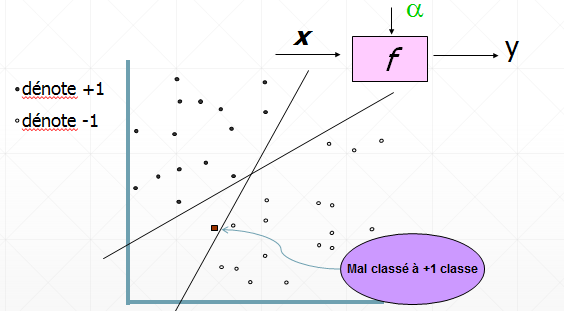
\includegraphics[scale=0.55]{9.png}
    \end{minipage}
\end{frame}

\begin{frame}{Séparation linéaire par SVM}
Un problème de discrimination est dit linéairement séparable lorsqu’il existe une fonction de décision linéaire (appelé aussi séparateur linéaire), de la forme:

\begin{center} D(x) = signe(f(x)) avec  f(x) = $w^{T}$ x + a  \end{center}


$ w\in\mathbb{R}^{p} $, classant correctement toutes les observations de l’ensemble d’apprentissage
D(x) =$y_{i}$,$ {i}\in[1,n] $, La fonction f est appelée fonction caractéristique.\vspace{2\baselineskip}


A toute fonction de décision et donc aux fonction de décision linéaire ont peut associer une frontière de décision :
 
\begin{center} \textcolor{red} {$\Delta$(w, a)=\{ $ x\in\mathbb{R}^{p} $ |$ w^{T}$x + a =0 \}} \end{center}                                       
\end{frame}

\begin{frame}{Séparation linéaire par SVM}
\textcolor{red}{Classificateurs Linéaires}
%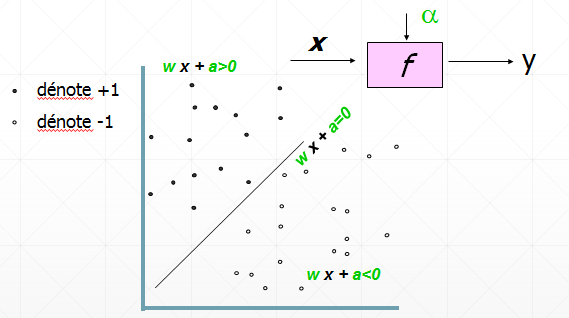
\includegraphics[scale=0.6]{5.png}
 
    \frametitle{ Séparation linéaire par SVM}
    \begin{minipage}{0.45\textwidth}
       \textcolor{blue}  {Hyperplan optimal doit maximiser la distance entre la frontière de séparation et les points de chaque classe qui lui sont le plus proche }. \vspace{2\baselineskip}
       
       
  \textcolor{brown} {Recherche d’un hyperplan de séparation optimal au sens de la marge maximale}.
    \end{minipage}
    \begin{minipage}{0.45\textwidth}
        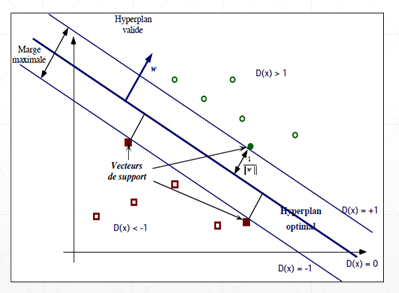
\includegraphics[scale=0.6]{10.png}
    \end{minipage}
\end{frame}

\begin{frame}{Séparation linéaire par SVM}
\textcolor{red}{  Principe de la maximisation de la marge}
\begin{itemize}
         \item  La distance d’un point à l’hyperplan est :
   
       $$d(x,\Delta)=\frac{ |w^{T}x + a|}{||w||} =\textcolor{red} {Marge}  .$$
         \item L’hyperplan optimal est celui pour lequel la distance aux points les plus proches est maximale.
         \item La marge entre les deux classes vaut $\frac{2}{||w||} $
          \item Maximiser la marge revient donc à minimiser ||w|| sous contraintes: \vspace{1\baselineskip} \\
     
$\left\{ \begin{array}{ll}
\min\limits_{w,a} \frac{1}{2} ||w||^2\\ 
\mbox{avec} \hspace{0.6 cm} y_i(w^{T}x_i+a)\geq 1, \forall i \in \{1,\cdots,n\}\\
\end{array}\right.$\\
\end{itemize}
\end{frame}
 
 \begin{frame}{Séparation linéaire par SVM}
\textcolor{red}{ Principe de la maximisation de la marge}
%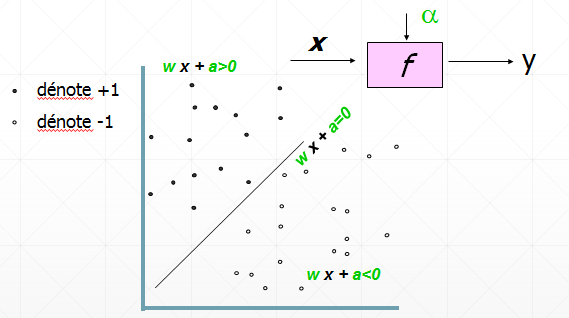
\includegraphics[scale=0.6]{5.png}
 
    \frametitle{Séparation linéaire par SVM }
    \begin{minipage}{0.4\textwidth}
 
        Les données qui vérifient l’égalité de la contrainte s’appellent les vecteurs supports, et ce sont ces données seules qui contribuent à la détermination de l’hyperplan.
    \end{minipage}
    \begin{minipage}{0.4\textwidth}
        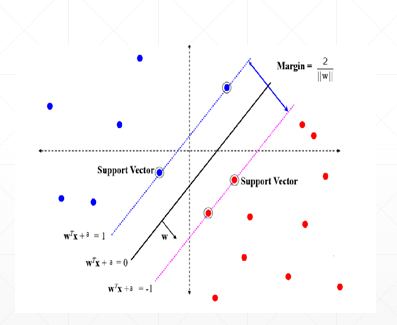
\includegraphics[scale=0.6]{12.png}
    \end{minipage}
\end{frame}

 \begin{frame}{Séparation linéaire par SVM}
\textcolor{red}{Résolution de la forme primaire du problème}\vspace{1\baselineskip} \\
    
    Le problème de l’équation est un problème de programmation quadratique avec contraintes linéaires. Dans ce problème, les variables sont w et a, c-à-d que le nombre de variables est égal à p + 1. 
    
    \begin{itemize} 
        \item \textcolor{blue} {Il faut régler p + 1 paramètres.}
         \item \textcolor{blue}{ Possible quand p est assez petit avec des méthodes d'optimisation quadratique.}
         \item \textcolor{blue}{ Impossible quand p est grand.}
\end{itemize}
\textcolor{red}{Transformation du problème d’optimisation }
    \begin{itemize} 
        \item Méthode des multiplicateurs de Lagrange:
        $\left\{ \begin{array}{ll}
L_p(w,a,\alpha)=\frac{1}{2}||w||^2 - \sum\limits_{i=1}^{n}\alpha_i [y_i *(w^{T}x_i+a)-1] \\
\forall i,\alpha_i \geq 0
\end{array}\right.$ \vspace{1\baselineskip} \\
  Où $\alpha_i$   sont les multiplicateurs de Lagrange 

       \end{itemize} 
\end{frame}

 \begin{frame}{Séparation linéaire par SVM}
\textcolor{red}{Expression duale Optimisation }\vspace{1\baselineskip} \\
    
 En introduisant les informations issues de l’annulation des dérivées partielles du Lagrangien, on obtient une optimisation ne dépendant que  des multiplicateurs
En remplaçant dans la fonction objective, on obtient le problème dual à maximiser suivant :
 
    $\max\limits_\alpha L_p(\alpha)= \sum\limits_{i=1}^{n}\sum\limits_{j}^{n} \alpha_i\alpha_j y_i y_j <x_i,x_j>$\\
s.c\\
$\left\{ \begin{array}{ll}
\alpha_i \geq 0, \forall i\\
\sum\limits_{i=1}^{n} \alpha_i y_i=0\\
\end{array}\right.$    \vspace{1\baselineskip} \\
d'ou \begin{itemize} 
        
       \item $\alpha_i \geq$ 0  vont définir les points importants c.à-d. les points supports \vspace{1\baselineskip} \\
       \item Forcément, il y aura des points supports d’étiquettes différentes sinon cette condition ne peut pas être respectée. \\
       \item   $<x_i,x_j>=x_i^{T}x_j$ : est le produit scalaire entre les observations i et j \\

     \end{itemize}
\end{frame}

\begin{frame}{Séparation linéaire par SVM}
\textcolor{red}{Solution du problème d’optimisation }\vspace{1\baselineskip} \\
\begin{itemize}
      \item $f(x)=\widehat{w}^{T}x+\widehat{a}$ \hspace*{0.3 cm}$=\sum\limits_{i=1}^{n}\alpha_i y_i <x_i,x>+a$ \hspace*{0.3 cm}$=\sum\limits_{j\in S}\alpha_j y_j <x_j,x>+a$\\

 \item  $\frac{\partial L}{\partial w} = w-\sum\limits_{i=1}^{n}\alpha_i y_i x_i =0  \Rightarrow \widehat{w} \sum\limits_{i=1}^{n}\alpha'_i y_i x_i$\\ 
      \item A partir des conditions de KKT,on peut obtenir:
A partir des conditions de KKT, on peut obtenir: $$\widehat{a}=\frac{1-y_i*w^{T}x_i}{y_i}$$
      \item D’un point de vue précision, on prend la moyenne de a pour tous les vecteurs supports :\\
      $$\widehat{a}=\frac{1}{||S||} \sum\limits_{i\in S}y_i  - w^{T}x_i$$\\ 
       \item La fonction de décision f peut être calculée: $f(x)= \sum\limits_{i=1}^{n}\alpha'_i y_i<x_i,x> +\widehat{a}$\\ 
    \end{itemize} 
\end{frame}

\begin{frame}{Séparation linéaire par SVM}
\textcolor{red}{Classement d’un individu supplémentaire}\vspace{1\baselineskip}
%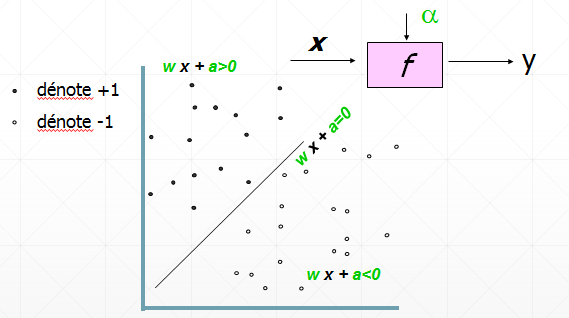
\includegraphics[scale=0.6]{5.png}
 
      La fonction de décision f peut être calculée, donc, pour chaque nouvel point x par la fonction f(x) et la décision peut être prise comme suit : \vspace{1\baselineskip}\\
      $\left\{ \begin{array}{lcc}
x\in classe +1 & si & f(x)>0\\
x\in classe -1 & si &f(x)< 0\\
 x \hspace*{0.1 cm} inclassifiable & si& f(x) =0\\
\end{array}\right.$\\
\begin{itemize}
      \item seuls les $\alpha_i$ des points les plus proches sont non-nuls : points de support  \\
      \item seuls interviennent les produits scalaires entre les observations x dans le problème d’optimisation. \\
\end{itemize}
L’hyperplan solution ne dépend que du produit scalaire entre le vecteur d’entrée et les vecteurs de support. Cette particularité permet l’utilisation de fonctions noyau pour aborder des problèmes non linéaires    
\end{frame}

\section{Séparation non linéaire par SVM}
\subsection{Cas non linéairement séparable }
\begin{frame}{Séparation non linéaire par SVM}
\textcolor{red}{Le cas non séparable}\vspace{1\baselineskip}\\
 Souvent il arrive que même si le problème est linéaire, les données sont affectées par un bruit (par ex. de capteur) et les deux classes se retrouvent mélangées autour de l’hyperplan de séparation. Pour gérer ce type de problème on utilise une technique dite de marge souple, qui tolère les mauvais classements :\\
\frametitle{Séparation non linéaire par SVM }
    \begin{minipage}{0.3\textwidth}
\begin{itemize}
      \item Rajouter des variables de relâchement des contraintes $\xi_i$.\\
      \item Pénaliser ces relâchements dans la fonction objectif.\\
\end {itemize} 
    \end{minipage}
    \begin{minipage}{0.3\textwidth}
        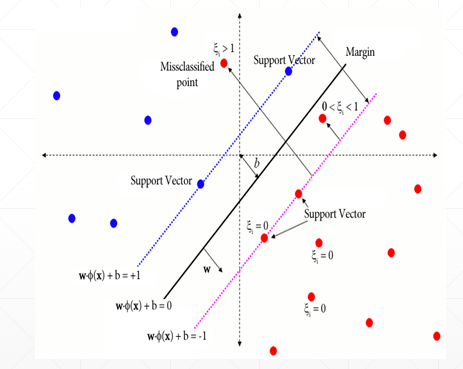
\includegraphics[scale=0.5]{14.png}
    \end{minipage}
\end{frame}

\begin{frame}{Séparation non linéaire par SVM}
\textcolor{red}{Le cas non séparable}\vspace{1\baselineskip}\\ 
Si un point ($ x_i,y_i$) vérifie la contrainte de marge $y_i*(w^{T}x_i+a)\geq 1$ alors la variable d’écart (qui est une mesure du coût de l’erreur) est nulle.Nous avons donc deux situations :\\
\frametitle{Séparation non linéaire par SVM }
    \begin{minipage}{0.45\textwidth}
    \begin{itemize}
      \item Pas d’erreur :\\
      $y_i*(w^{T}x_i+a)\geq 1    \Rightarrow   \xi_i =0$\\.
      \item Erreur: \\
      $y_i*(w^{T}x_i+a)1-\xi_i    \Rightarrow   \xi_i=1-y_i*(w^{T}x_i+a) $.\\
      \item $\xi_i=max(0,1-y_i*(w^{T}x_i+a)$.\\ 
\end {itemize}
\end{minipage}
    \begin{minipage}{0.45\textwidth}
        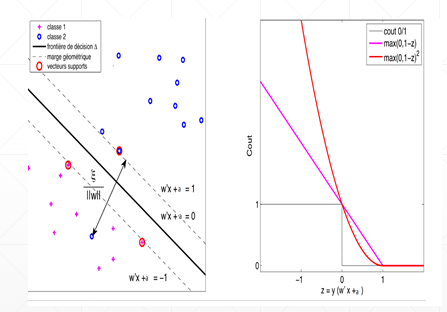
\includegraphics[scale=0.55]{15.png}
    \end{minipage}
\end{frame}

\begin{frame}{Séparation non linéaire par SVM}
\textcolor{red}{Le cas non séparable}\vspace{1\baselineskip}\\
Le problème d’optimisation dans le cas des données non-séparables est donc :\\ 
$\left\{ \begin{array}{l}
min \frac{1}{2} ||w||^2\\
\sum\limits_{i=1}^{n} \xi_i\\
\end{array}\right.$\\
Tel que:\\
$\left\{ \begin{array}{l}
y_i*(w^{T}x_i+a)  \geq 1-\xi_i\\
\xi_i \geq 0 \hspace*{0.1 cm} \forall i \in \{1, \cdots, n\}\\
\end{array}\right.$ \vspace{1\baselineskip}\\
Puisqu’il faut minimiser les deux termes simultanément, on introduit une variable d’équilibrage C>0 qui permet d’avoir une seule fonction objectif dans le problème d’optimisation : \\
$\min\limits_{w,a}\frac{1}{2} ||w||^2+ C^{*}\sum\limits_{i=1}^{n} \xi_i$\\
 Tel que:\\
$\left\{ \begin{array}{l}
y_i*(w^{T}x_i+a)\geq  1 -\xi_i\\
\xi_i \geq 0 \hspace*{0.3 cm} \forall i \in \{1, \cdots, n\}\\
\end{array}\right.$\\
\end{frame}

\begin{frame}{Séparation non linéaire par SVM}
\textcolor{red}{Le cas non séparable}\vspace{1\baselineskip}\\
Par la même procédure qu’avant, on obtient le problème dual :\\
$\max\limits_{\alpha} L\alpha_p(\alpha) = \sum\limits_{i=1}^{n} \alpha_i -\frac{1}{2}\sum\limits_{i=1}^{n}\sum\limits_{j=1}^{n}\alpha_i\alpha_j y_i y_j <x_i,x_j>$\\
s.c:\\
$\left\{ \begin{array}{ll}
\sum\limits_{i=1}^{n} \alpha_i y_i =0 & \mbox{(stationarité)}\\
0 \leq \alpha_i \leq C, \forall i \in \{1, \cdots, n\} & \mbox{(admissibilitéduale)}\\
\end{array}\right.$\\
La fonction de décision permettant de classer une nouvelle observation x est toujours:\\
  $f^{*}(x)= \sum\limits_{i=1}^{n}\alpha_i^{*} y_i<x_i,x> +a^{*}$\\ 
  \textcolor{red}{Observations:}\\
      \begin{itemize}
      \item La différence pour le problème dual entre le cas séparable et non séparable est que les valeurs des $\alpha_i$ sont majorées par C.\\
      \item Les points mal classés ou placés dans la marge ont un $\alpha_i$=C.
      \item a est calculé de sorte que $y_i*f(x_i)$=1 pour  les points tels que C>$\alpha_i$>0

\end{itemize}
 
\end{frame}
\subsection{Les noyaux}
\begin{frame}{Séparation non linéaire par SVM}
\textcolor{red}{Le cas non linéaire : les noyaux }\vspace{1\baselineskip}\\
     \begin{itemize}
      \item Les jeux de données qui peuvent être séparés linéairement avec du bruit sont parfaits:\\
 \begin{center} 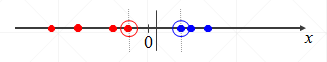
\includegraphics[scale=0.6]{16.png} \end{center}
      \item Mais qu'allons-nous faire si l'ensemble de données est trop difficile? \\ 
    \begin{center} 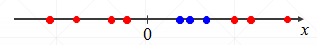
\includegraphics[scale=0.6]{17.png} \end{center} 
    \item Que diriez-vous de… mapper les données dans un espace de plus grande dimension:\\
       \begin{center} 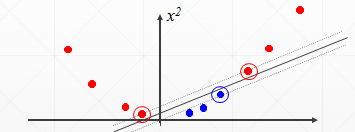
\includegraphics[scale=0.6]{18.png} \end{center} 
\end{itemize}
\end{frame}

\begin{frame}{Séparation non linéaire par SVM}
\textcolor{red}{Changement de représentation }\vspace{1\baselineskip}\\
En réalisant les transformations de variables adéquates, on peut rendre linéairement séparable un problème qui ne l’est pas dans l’espace initial.\\
     \begin{center} 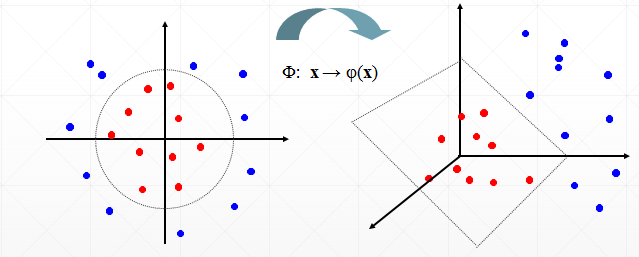
\includegraphics[scale=0.6]{19.png} \end{center} 
 \end{frame}

\begin{frame}{Séparation non linéaire par SVM}
Dans le cas général, la frontière optimale est non linéaire. Dans le cadre des SVM, la prise en compte de non linéarités dans le modèle s’effectue par l’introduction de noyaux non linéaires.Des exemples typiques de noyaux sont le noyaux polynômial\\
$k(x,x')=(C+(x,x'))^p$  et le noyau gaussien $k(x,x')=e^{\frac{||x-x'||^2}{2\sigma^2}}$.\\
Etant donné le noyau k, la fonction de décision s’écrit D(x) = signe(f(x) + a)et:\\
\begin{itemize}
      \item Cas linéaire:         $f(x)=\sum\limits_{i \in S} \alpha_i y_i x^{T}_i x$\\
      \item Cas non linéaire:     $f(x)=\sum\limits_{i \in S} \alpha_i y_i k(x_i,x) $\\
 \end{itemize}     
La fonction de discrimination est une combinaison linéaire des noyaux dont le signe de l’influence dépend de la classe. L’ensemble actif S, les coefficients $\alpha_i$ associés et le biais a sont donné par la résolution du même problème dual que dans le cas des SVM linéaires . Seule la définition de la matrice G change (mais pas sa taille):\vspace{1\baselineskip}\\
\begin{itemize}
      \item Cas linéaire:        $G_{ij} = y_i y_j x^{T}_i x_j$\\
      \item Cas non linéaire:    $G_{ij} = y_i y_j k(x_i,x_j)$
 \end{itemize}
 \end{frame}
 
 \begin{frame}{Séparation non linéaire par SVM} 
 L’idée ici est de considérer dans le dual l’influence de chacune des observations dans la construction de la solution. Le calcul de cette influence passe par la résolution d’un programme quadratique de taille n. L’utilisation de noyaux permet d’introduire de la non linéarité sans modifier la complexité algorithmique du problème à résoudre
 \begin{itemize}
      \item \textcolor{red}{les noyaux:}  un noyau k est défini de manière générale comme une fonction de deux variables sur $\mathbb{R}$:\\ 
 $ \hspace*{1.5 cm} k:X \times X \rightarrow \mathbb{R}$ \hspace*{1.5 cm} $(x,x')\mapsto k(x,x')$\\

      \item \textcolor{red} {Matrice de Gram:} La matrice de Gram du noyau k(., .) pour les observations ($x_{1}$,$x_{2}$,…,$x_{n}$)est la matrice carrée K de taille n et de terme général $k_{ij}=k(x_i,x_j)$\\
      \item \textcolor{red}{Noyau positif:}  Un noyau k est dit positif si, pour tout entier n fini et pour toutes les suite de n observations possibles {$x_i$ ,i = 1,n}, la matrice de Gram associée est une matrice symétrique définie positive. L’intéret des noyaux positifs c’est qu’il est possible de leur associer un produit scalaire.
      \item \textcolor{red}{Construction des noyaux:} Il existe deux façons de construire un noyau positif :
 \end{itemize}
\end{frame}

 \begin{frame}{Séparation non linéaire par SVM}
\textcolor{red}{1.} soit on s’appuie sur une transformation $\Phi(x)$ de X sur un espace H muni d’un produit scalaire et l’on défini le noyau à travers ce produit scalaire :\vspace{1\baselineskip}\\
  \textcolor{red}{$ \hspace*{2.5 cm} k(x,x')= <\Phi(x),\Phi(x')>_H$} \vspace{1\baselineskip}\\
 \textcolor{red}{2.} soit on utilise les propriétés algébriques des noyaux positifs:
 \begin{itemize} 
    \item un noyau séparable est un noyau positif
    \item la somme de deux noyaux positifs est un noyau positif,
    \item le produit de deux noyaux positifs est un noyau positif
    \item le produit tensoriel ainsi la somme directe de deux noyaux positifs est un noyau positif 
    \item le passage à la limite conserve la positivité : si la limite d’une suite de noyaux positif existe, c’est aussi un noyau positif.
       \end{itemize}
\end{frame}

\subsection{Fonctions noyau pour des vecteurs}
 \begin{frame}{Séparation non linéaire par SVM}
 \begin{itemize} 
    \item \textcolor{blue}{Noyaux polynomiaux:} \vspace{1\baselineskip}\\
      $k_{poly1}(x,z)=(x^{T}z)^d$ Tous les produits d’exactement
d variables.\vspace{1\baselineskip}\\
     $k_{poly2}(x,z)=(x^{T}z+c)^d$ Tous les produits d’au plus
d variables.\vspace{2\baselineskip}\\
    \item \textcolor{blue}{Noyaux gaussiens:} \vspace{1\baselineskip}\\
    $k_{G}(x,z)= exp(-\frac{d(x,z)^1}{2\sigma^2})$ Sorte de décomposition
en série de Fourrier.\vspace{2\baselineskip}\\
    \item \textcolor{blue}{Noyaux sigmoïdes:} \vspace{1\baselineskip}\\
    $k(x,z)= tanh(kx^{T}z+\theta$ Pas définie positive.Mais fonction de décision proche des réseaux connexionnistes.\\
    \end{itemize}
 \end{frame}
 
 
 \section{Séparation dans le cas SVR}
  \begin{frame}{Support Vector Regression}
  De la même manière que l'approche de classification, il existe une motivation pour rechercher et optimiser les limites de généralisation données pour la régression. Ils se sont appuyés sur la définition de la fonction de perte qui ignore les erreurs, situées à une certaine distance de la valeur réelle. Ce type de fonction est souvent appelé - fonction de perte intensive - epsilon.\vspace{1\baselineskip}\\
   \frametitle{support vector regression }
\begin{minipage}{0.3\textwidth}
Utilisation de la fonction de perte intensive epsilon, nous assurons l'existence du minimum global et en  même temps l'optimisation avec support de généralisation fiable.\vspace{1\baselineskip}\\
 Le paramètre $\epsilon$ contrôle la largeur de la zone-insensitive, utilisé pour ajuster les données de formation.

\end{minipage}
    \begin{minipage}{0.3\textwidth}
    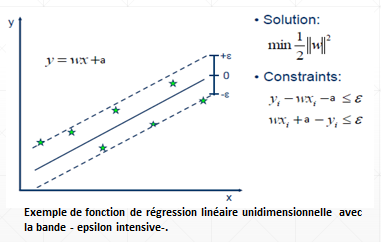
\includegraphics[scale=0.7]{24.png}
    \end{minipage}
 \end{frame}
 
 
 \subsection{Le cas linéaire}
   \begin{frame}{support vector regression}
   \textcolor{blue}{SVR linéaire:}\vspace{1\baselineskip}\\
            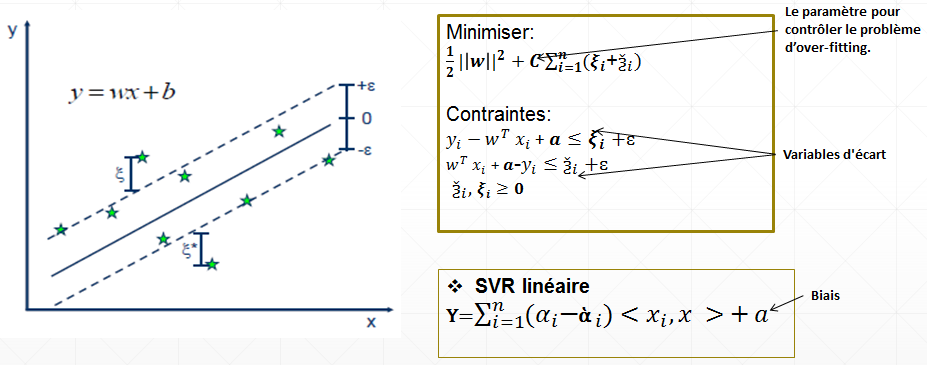
\includegraphics[scale=0.45]{25.png}

 \end{frame}
 \subsection{Le cas non linéaire}
   \begin{frame}{support vector regression}
     \textcolor{blue}{SVR non linéaire:}\vspace{1\baselineskip}\\
Les fonctions du noyau transforment les données en un espace de fonctions de dimension supérieure pour permettre la séparation linéaire.
     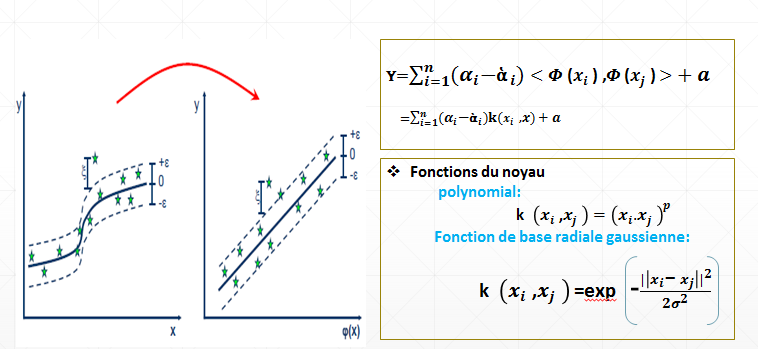
\includegraphics[scale=0.54]{26.png}

 \end{frame}
 
 \section{Simulation}
  \subsection{Bibliothèques}
     \begin{frame}{Simulation}
     \begin{itemize}
        \item \textcolor{blue}{pandas:} Pour importer les données ‘csv’ et les manipuler \vspace{1\baselineskip}\\
         \item \textcolor{blue}{numpy:} Pour les calculs matricielle \vspace{1\baselineskip}\\
           \item  \textcolor{blue}{matplotlib.pyplot:}  Pour l’affichage des figures\vspace{1\baselineskip}\\
            \item  \textcolor{blue}{Scikit-learn (sklearn):}  est une bibliothèque libre dans Python destinée à l'apprentissage automatique.\vspace{1\baselineskip}\\
   \end{itemize}
     \end{frame} 
 \subsection{Dataset}   
   \begin{frame}{Simulation}
 Les données ont été extraites des images qui ont été prises pour l'évaluation d'une procédure d'authentification des billets de banque. \textcolor{red}{Wavelet Transform tool}. \vspace{1\baselineskip}\\
 5 variables et 1372 individus.\vspace{1\baselineskip}\\
 \frametitle{Simulation }
\begin{minipage}{0.3\textwidth}
     \begin{itemize}
        \item Variance de l'image transformée en ondelettes\\

        \item Asymétrie de l'image transformée en ondelettes\\

        \item Curtose de l'image transformée en ondelettes\\
            \item Entropie d'image\\
            \item Classe \\
\end{itemize}
    \end{minipage}
    \begin{minipage}{0.3\textwidth}
    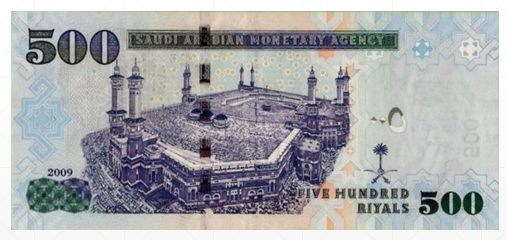
\includegraphics[scale=0.6]{20.png}
    \end{minipage}
 \end{frame}

   \begin{frame}{Simulation}
   
   \vfill
\begin{center}  
\includegraphics[scale=0.25]{28.jpg} \end{center}
\vfill
 
   \end{frame}
 \section{Conclusion}

   \begin{frame}{Conclusion}
Dans cette présentation, nous avons couvert de nombreux sujets sur l'algorithme de machine à vecteurs de support, son fonctionnement, les noyaux, le réglage de l'hyperparamètre, la construction de modèles et l'évaluation de jeux de données de billets de banque à l'aide du package Scikit-learn.\vspace{1\baselineskip}\\
  \textcolor{red}{Les avantages:}
  \begin{itemize} 
   \item SVM fonctionne bien avec une marge de séparation nette et un espace dimensionnel élevé.\\
      \item Toujours efficace dans les cas où le nombre de dimensions est supérieur au nombre d'échantillons.\\
      \item Utilise un sous-ensemble de points d’entraînement dans la fonction de décision (appelés vecteurs de support), ce qui en fait une mémoire efficace.\vspace{1\baselineskip}\\
      \end{itemize}
      
    \textcolor{red}{Les inconvénients:} 
    \begin{itemize} 
   \item SVM ne convient pas pour les grands ensembles de données en raison de son temps de formation et il prend plus de temps dans la formation.\\
   \item SVM fonctionne mal avec des classes qui se chevauchent et est également sensible au type de noyau utilisé.\\

  
  
  
 \end{itemize}
  \end{frame}
  
 
  \begin{frame}{Réferences}
 \begin{itemize}   
  \item http: //www-lium.univ-lemans.fr/~barrault/cours/m1-aan/m1-aan-2016-svm.pdf.\vspace{1\baselineskip}\\
  \item http://eric.univ-lyon2.fr/~ricco/cours/slides/svm.pdf.\vspace{1\baselineskip}\\
  \item  http://www.math.univ-toulouse.fr/~besse/Wikistat/pdf/st-m-app-svm.pdf.\vspace{1\baselineskip}\\
   \item http://pageperso.univ-lr.fr/arnaud.revel/MesPolys/SVM.pdf.\vspace{1\baselineskip}\\
     \item https://www.quora.com/What-is-the-difference-between-Support-Vector-Machine-and-Support-Vector-Regression\vspace{1\baselineskip}\\
   \item https://www.datacamp.com/community/tutorials/svm-classification-scikit-learn-python\vspace{1\baselineskip}\\
      \item http://www-igm.univ-mlv.fr/~dr/XPOSE2014/Machin-Learning/D-Machine-Learning.html\vspace{1\baselineskip}\\
         \item https://dataanalyticspost.com/Lexique/svm/\vspace{1\baselineskip}\\

\end{itemize}
  \end{frame}


\end{document}

